\begin{frame}
\frametitle{Scale free graphs as a representation of a social network}

The transitivity and homophily particularities of social networks gives us guidelines for building a scale free graph. 
Then we build the line graph of this scale free graph.

\begin{figure}[H]
\begin{center}
    \begin{subfigure}[b]{0.4\textwidth}
        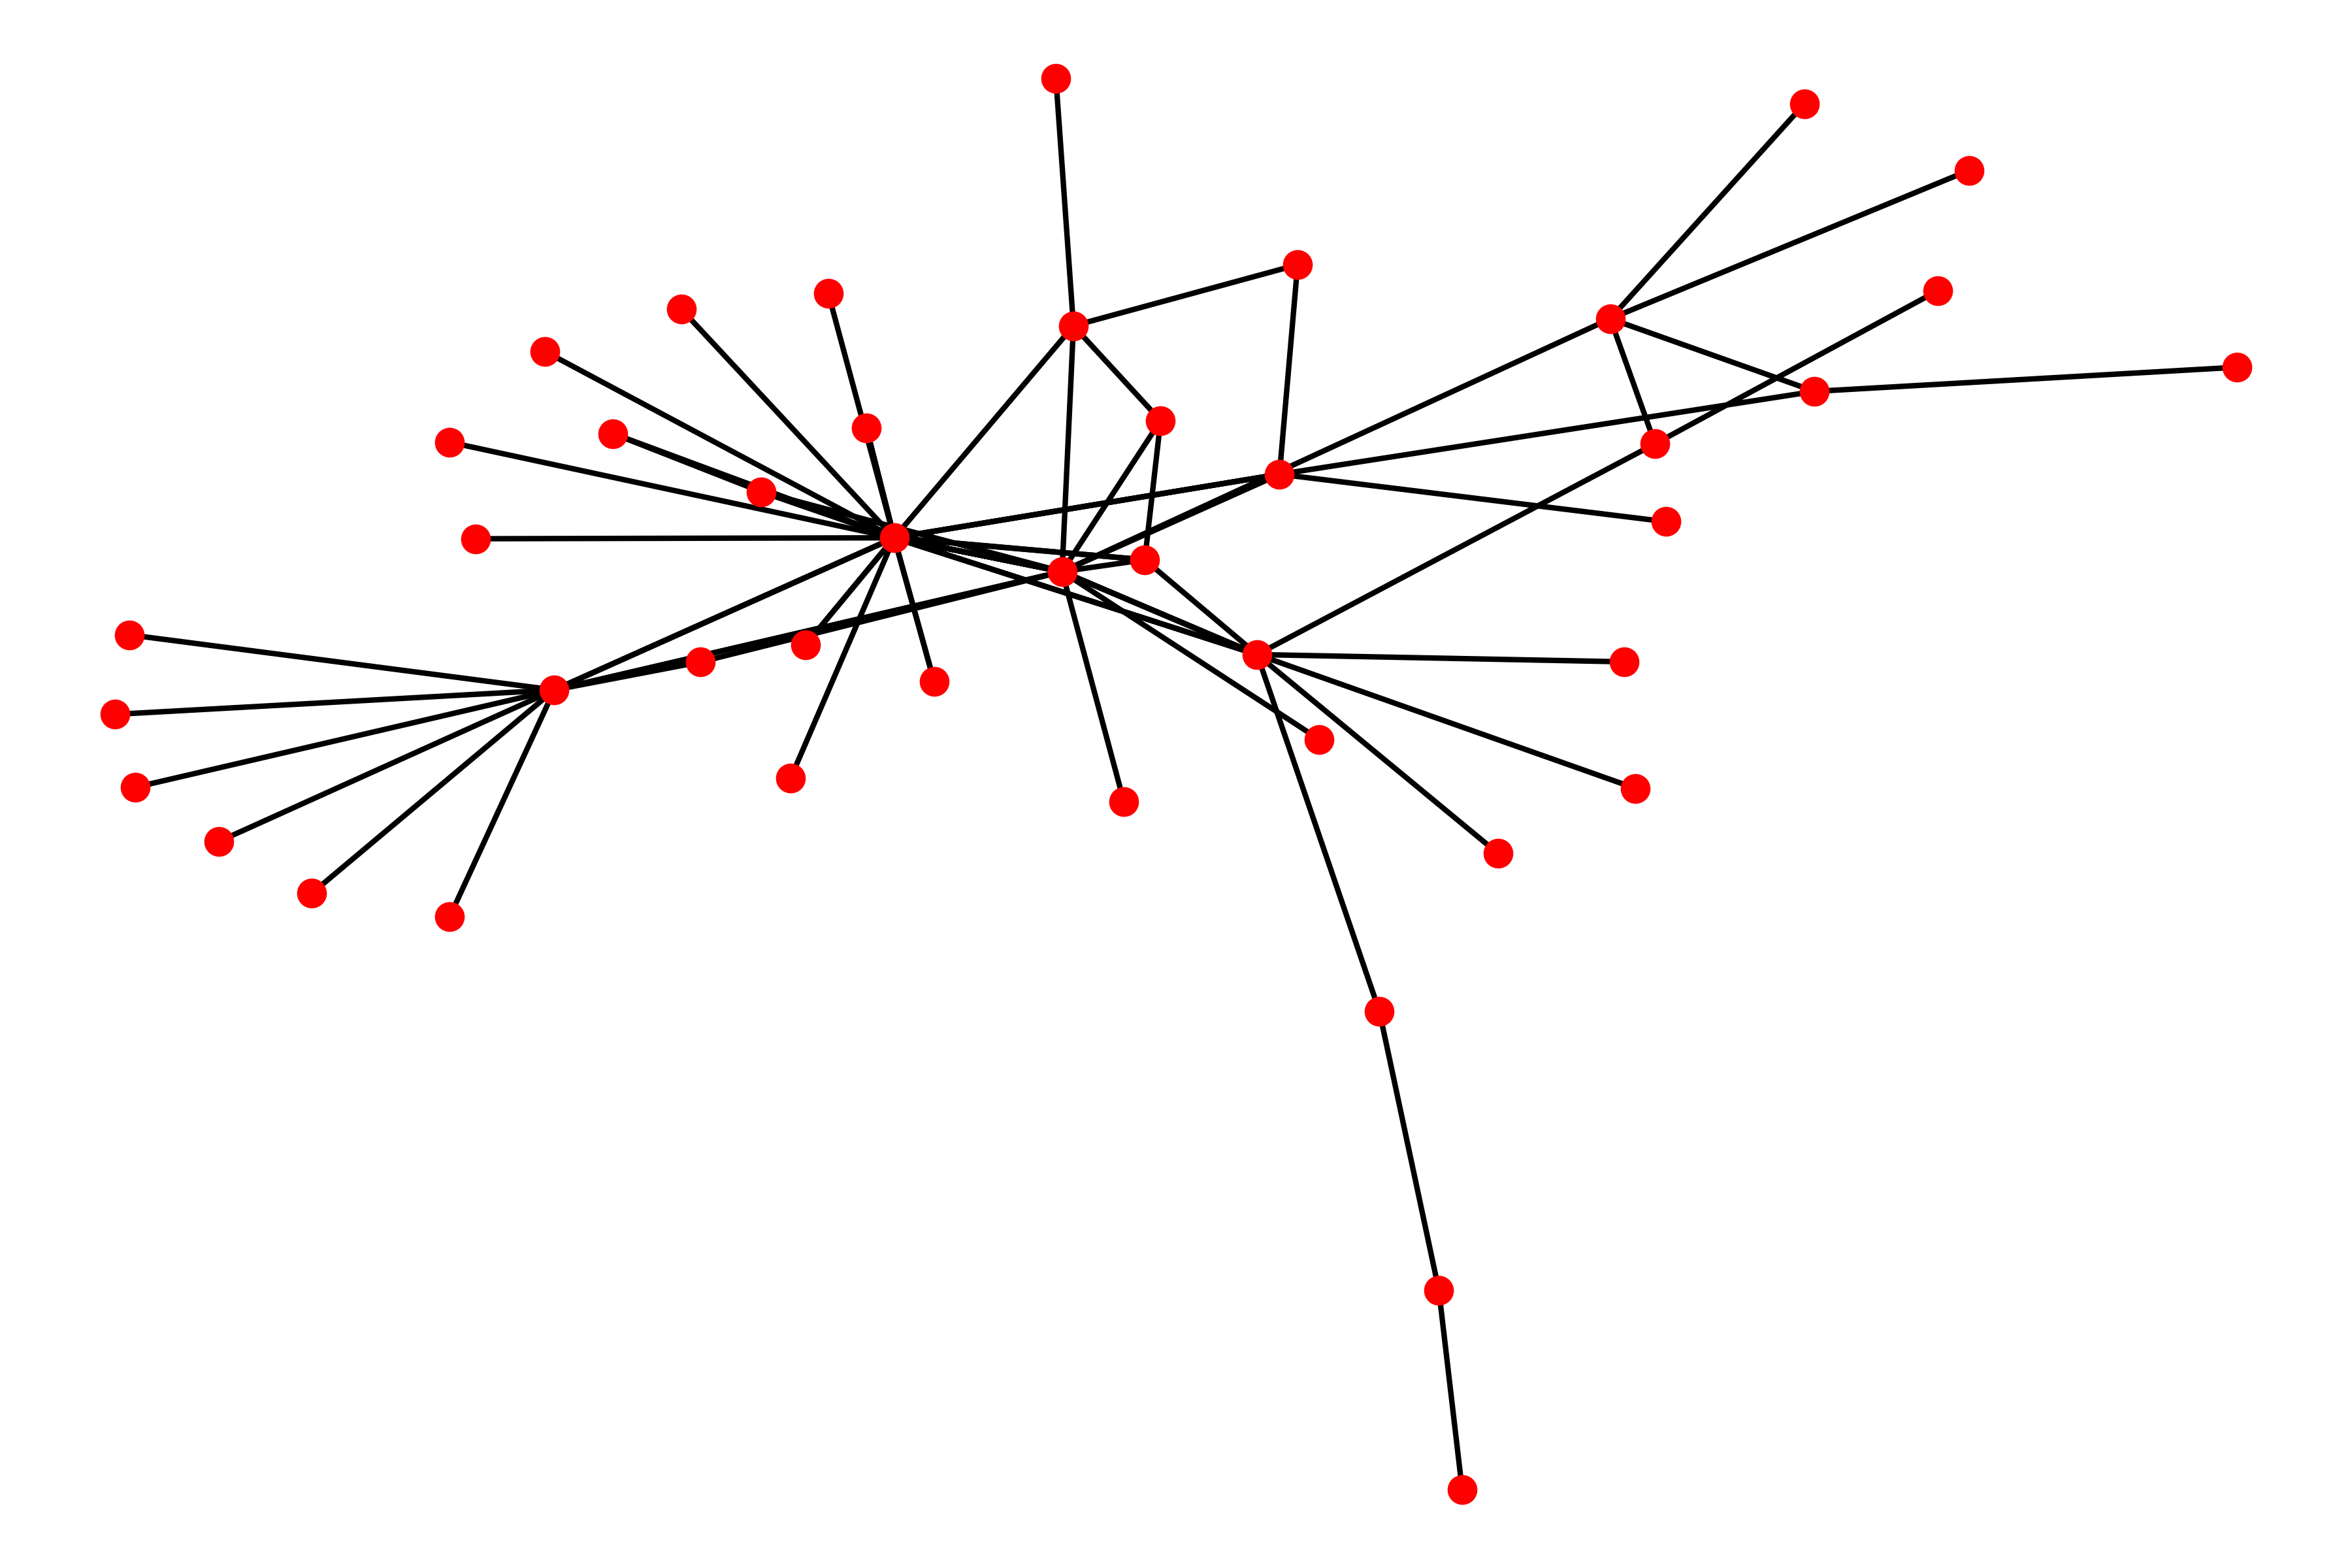
\includegraphics[width=\textwidth]{graphScaleFree.png}
        \caption{Scale free network}
        \label{fig:Scalefree}
    \end{subfigure}
    \begin{subfigure}[b]{0.4\textwidth}
        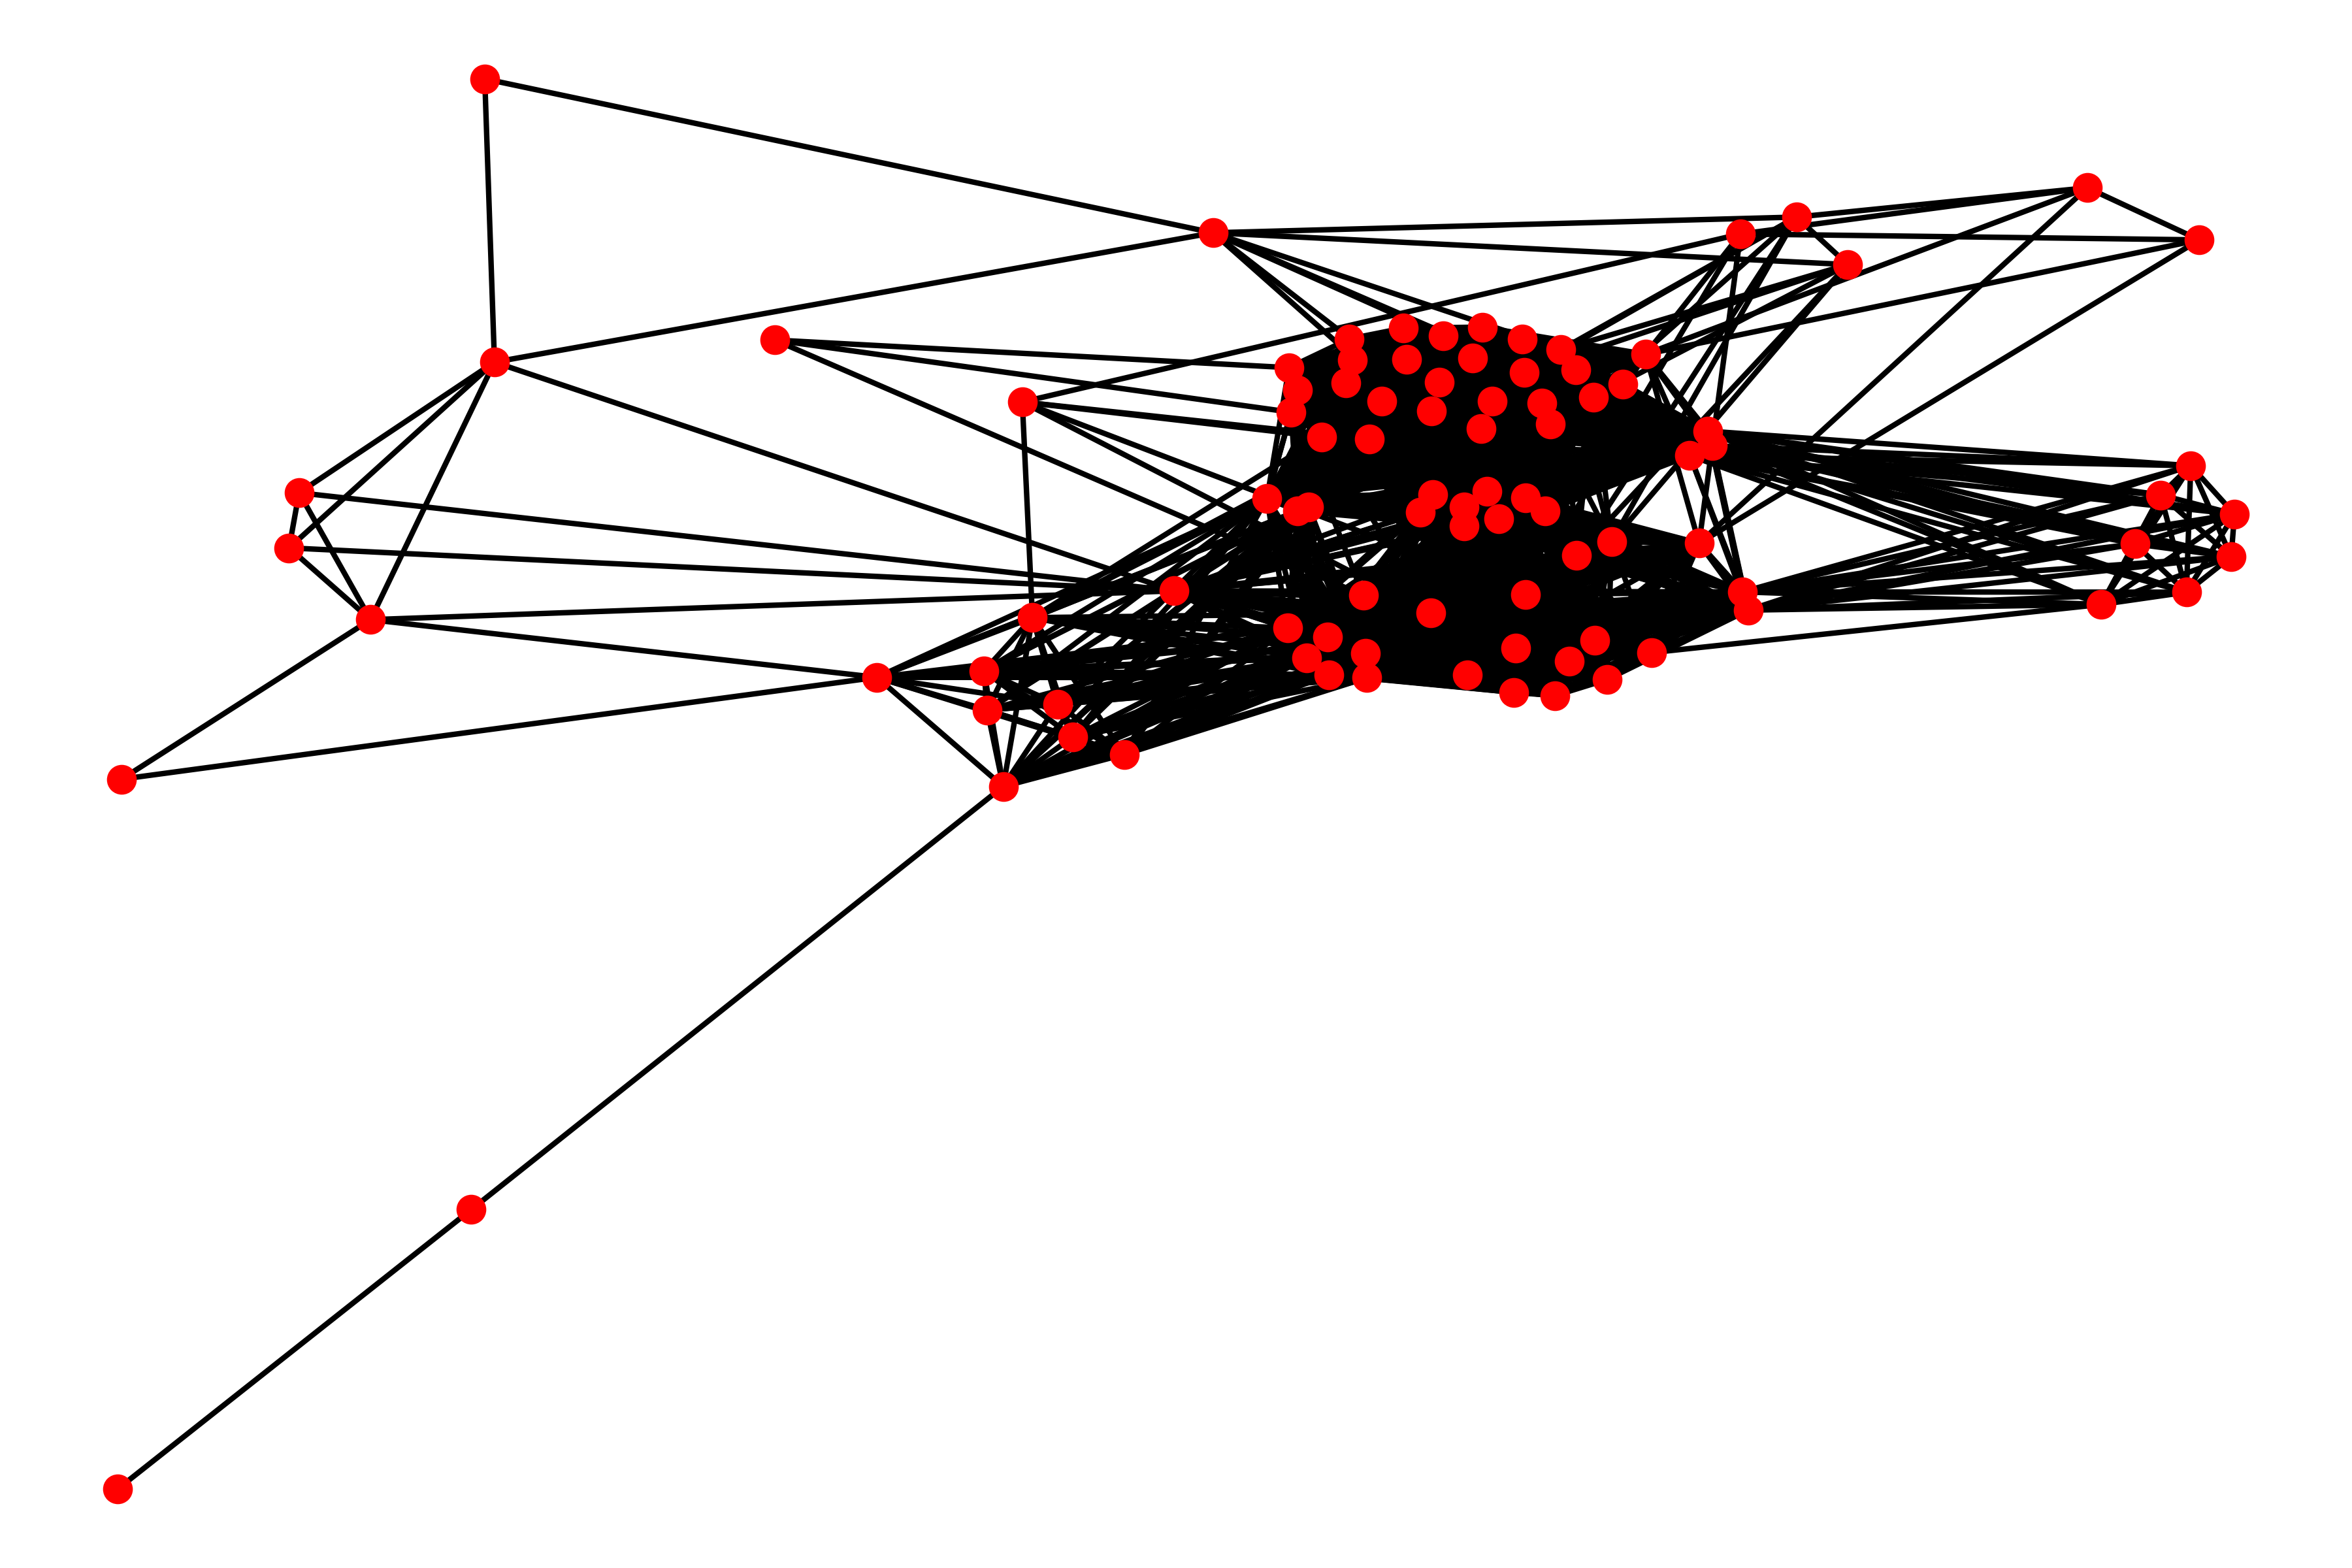
\includegraphics[width=\textwidth]{graphLineScaleFree.png}
        \caption{Line graph of the scale free network}
        \label{fig:lineG}
    \end{subfigure}
\label{fig:RelationshipScaleFree}
\end{center}
\end{figure}

\end{frame}

% ----------------------------------------------------------------------------------------

\begin{frame}
\frametitle{Results}

\begin{figure}[H]
\begin{center}
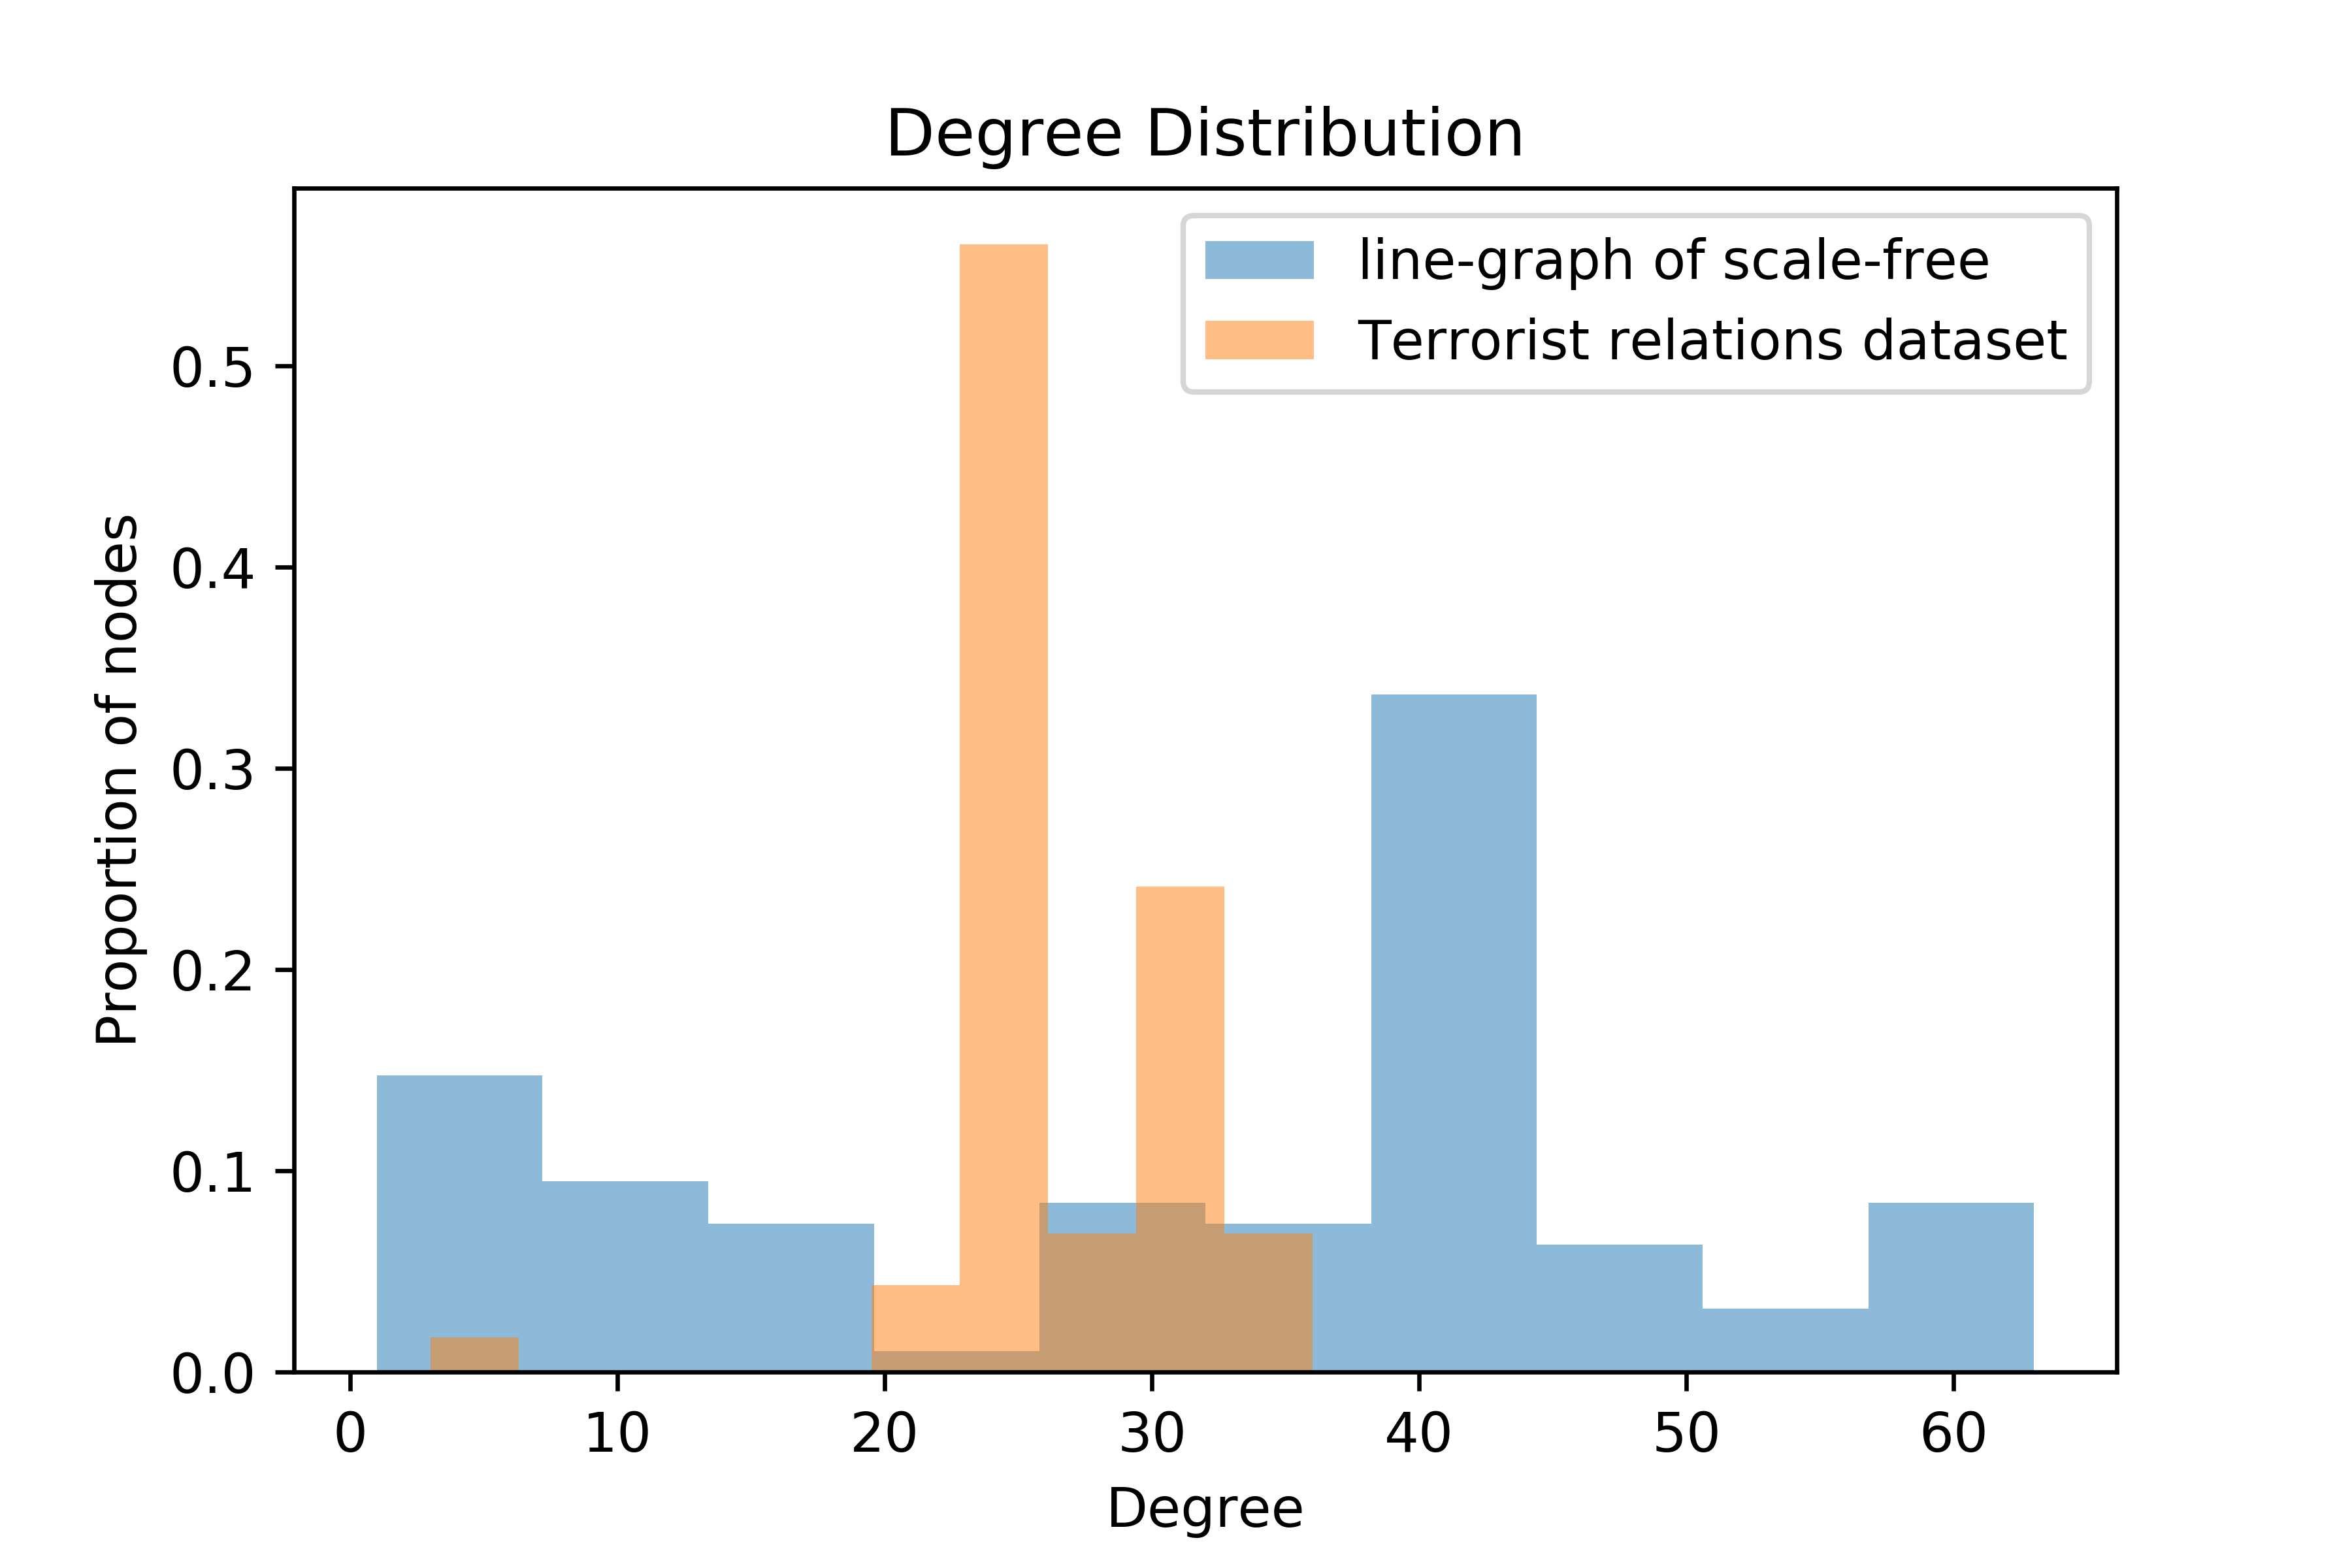
\includegraphics[width=.5\textwidth]{DegreeDiff.png}
\caption{Difference of degree distribution between the dataset and the generated line graph}
\label{fig:degdiff}
\end{center}
\end{figure}

Preliminary conclusion: The relationship network cannot be modeled by the line graph of a scale free network
\begin{itemize}
\item This could be because the relations of terrorist are not similar to social ties
\item Possibly because the size of the largest component is too small, making an unrealistically small number of relationships for the scale free graph to represent correctly a social network.
\end{itemize}

\end{frame}

% ----------------------------------------------------------------------------------------